%% -*- coding: utf-8 -*-
\documentclass[12pt,pagesize,paper=192mm:108mm]{scrbook} 
%1920x1080 1280x720
\areaset[current]{192mm}{108mm}
\usepackage{calc}
\usepackage[T2A]{fontenc}
\usepackage[utf8]{inputenc}
\usepackage[english,russian]{babel}
\usepackage{microtype}
\usepackage{misccorr}
\usepackage{cmap}
%\usepackage[unicode=true]{hyperref}
\usepackage{graphicx}
\usepackage{amssymb}
\usepackage{amsmath}
%\usepackage{srcltx}
\usepackage{textcomp}
\usepackage{xspace}
%научные символы и смайлики \smiley \frownie
\usepackage{wasysym}
\usepackage{ccicons}
\begin{document}
\begin{titlepage}
  \vspace*{-0.5em}
  \begin{center}    
    \hspace*{3em}
    \begin{minipage}[t]{3em}
      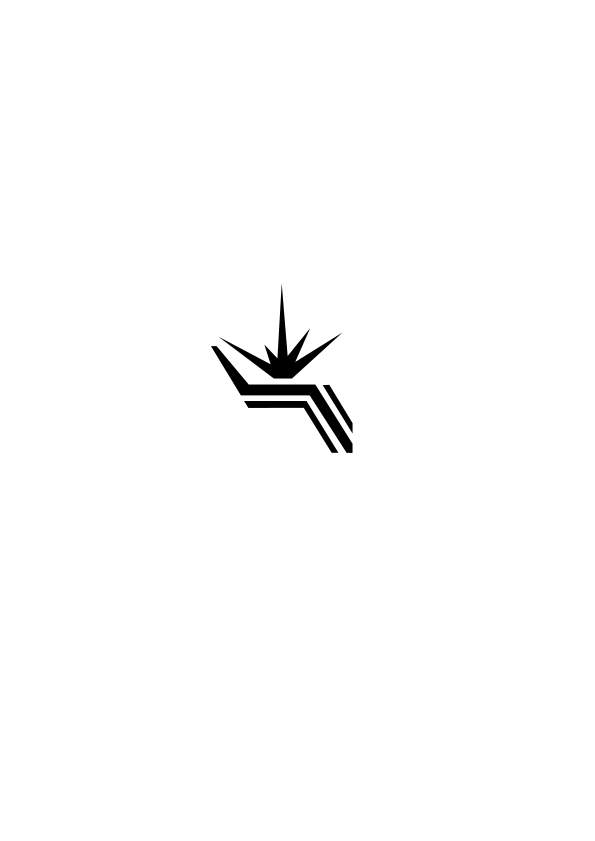
\includegraphics[width=\textwidth]{../BINP-logo}
    \end{minipage}\hfill
    \begin{minipage}{0.23\linewidth}
    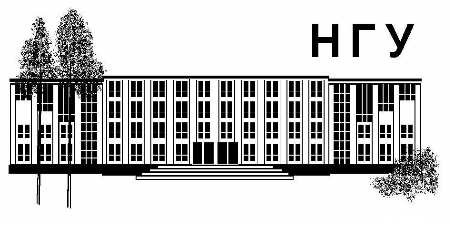
\includegraphics[width=\textwidth]{../NSU-logo}
    \end{minipage}
    \hfill
    \hspace*{6em}

    Кафедра теоретической физики физического факультета НГУ
    \medskip

    \Large
    Профессор Фадин В.\,С.
    \bigskip

    \huge
    \textbf{Квантовая электродинамика}
    \bigskip

    \Large
    Лекция № 12
    \vfill

    \normalsize
    % \begin{minipage}{0.65\linewidth}
    % \end{minipage}
    \vfill

    \normalsize \ccbysa\hspace{0.5em}  Новосибирск 2013
  \end{center}
\end{titlepage}
\vspace*{-1em}
\begin{center}
\vfill
  \begin{minipage}{0.85\linewidth}
    Радиационные поправки. Инфракрасные и ультрафиолетовые
    расходимости петлевых интегралов. Физически наблюдаемые значения
    массы и заряда и «голые» параметры, входящие в лагранжиан,
    процедура перенормировки. Перенормируемые и неперенормируемые
    теории. Одночастично неприводимые диаграммы. Функция Грина,
    ампутированная функции Грина, полная функция Грина. Двухточечные
    функции Грина: пропагаторы, собственноэнергетическая часть,
    массовый оператор. Массовый оператор для электрона.
    Поляризационный оператор фотона. Индекс расходимости
    диаграмм. Размерность ампутированной функции Грина и амплитуды в
    КЭД, связь с безразмерностью константы связи. Ультрафиолетово
    расходящиеся диаграммы в КЭД. Полная функция Грина для
    электрона. Полная функция Грина для фотона, поперечная и
    продольная часть поляризационного оператора. Способы регуляризации
    ультрафиолетовых расходимостей.  Перенормировка на массовой
    поверхности, физическая масса электрона как полюс пропагатора,
    перенормированный массовый оператор электрона, константа
    перенормировки $Z_2$. Калибровочная инвариантность и безмассовость
    фотона при перенормировке, перенормированный поляризационный
    оператор, константа перенормировки $Z_3$.  Перенормировка
    вершинной функции, константа перенормировки
    $Z_1$. Перенормированный заряд электрона.
  \end{minipage}
  \vfill

  % \normalsize \ccbysa\hspace{0.5em} Новосибирск 2013
\end{center}
\end{document}
